In this section it is presented the different interactions between the system and their actors in form of use cases. It is important to refer that there are two main actors: the designer and the user. The designer must own technical skills since it is the one associated with the creation/development of the system. The other entity is the user, and as the name suggests, it is the one that uses the application for generation of final embedded software systems.


\subsubsection{Dynamic Binary Translator}

Figure \ref{fig:DBTUseCases} shows the use cases scenario created for the main system: the DBT.

\begin{figure}[!htb]
\centerline{
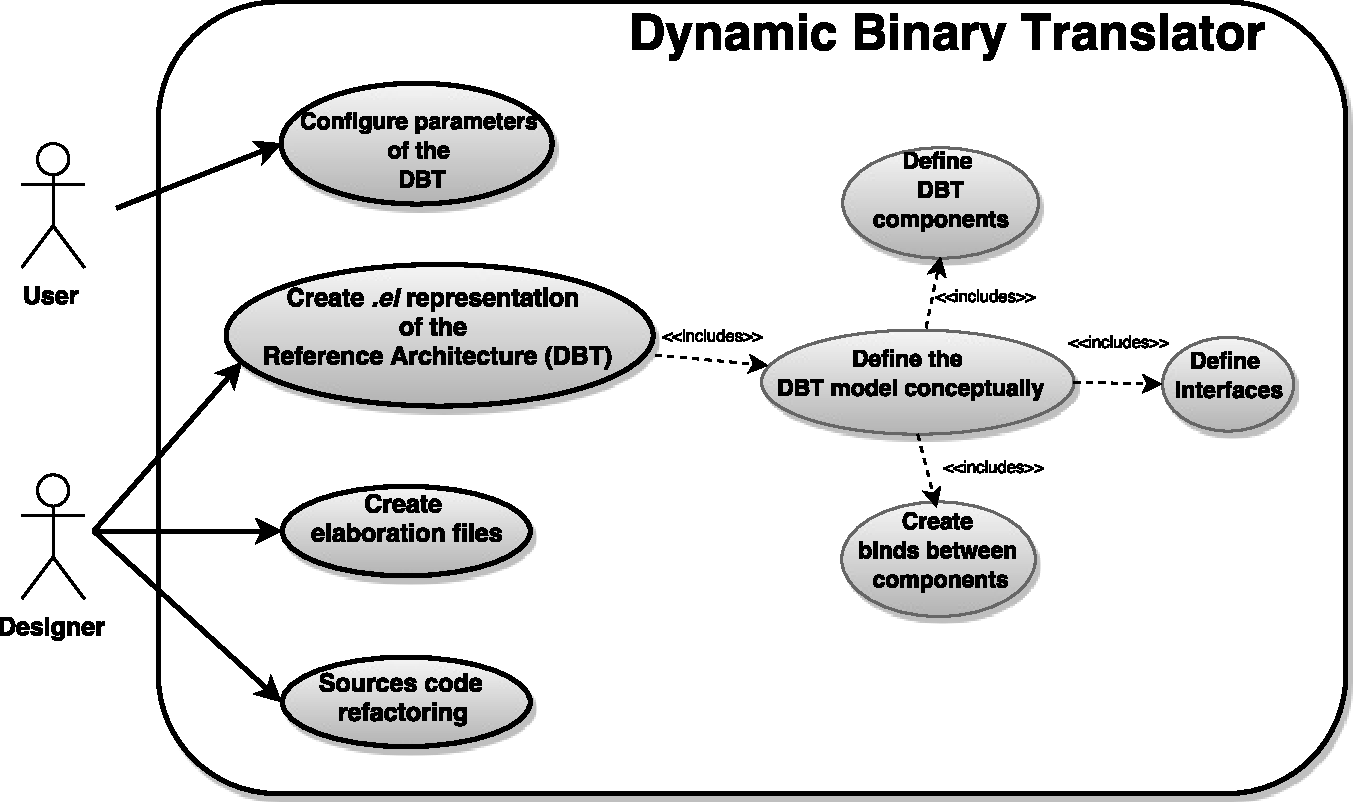
\includegraphics[scale=0.6]{images/DBT_UseCases.pdf} }
\caption{DBT Use Cases.}
\label{fig:DBTUseCases} 
\end{figure}

Since the \textit{EL Framework} is the tool used to model the DBT, a \textit{.el} file containing the reference architecture must be created. But first, to accomplish that task, the model should be well defined conceptually before materialize it in code. So the designer's job must pass through the definition of all the components, as well as the bindings between them. In a certain way, the decision of the bindings leads to the specification of the interfaces. Also, the designer creates the elaboration files for each component and, if required, a refactoring of the source code might be done. This code modification is necessary in situations where there are no compatibility between the model and the code. In the other hand, the user just need to configure some system's parameters, according to his preferences, resulting in a final project with all the code of a customized dynamic binary translator.

\subsubsection{Decoder}

This use case figure was created to show the role of the designer and user for Decoder component. 

\begin{figure}[!htb]
\centerline{
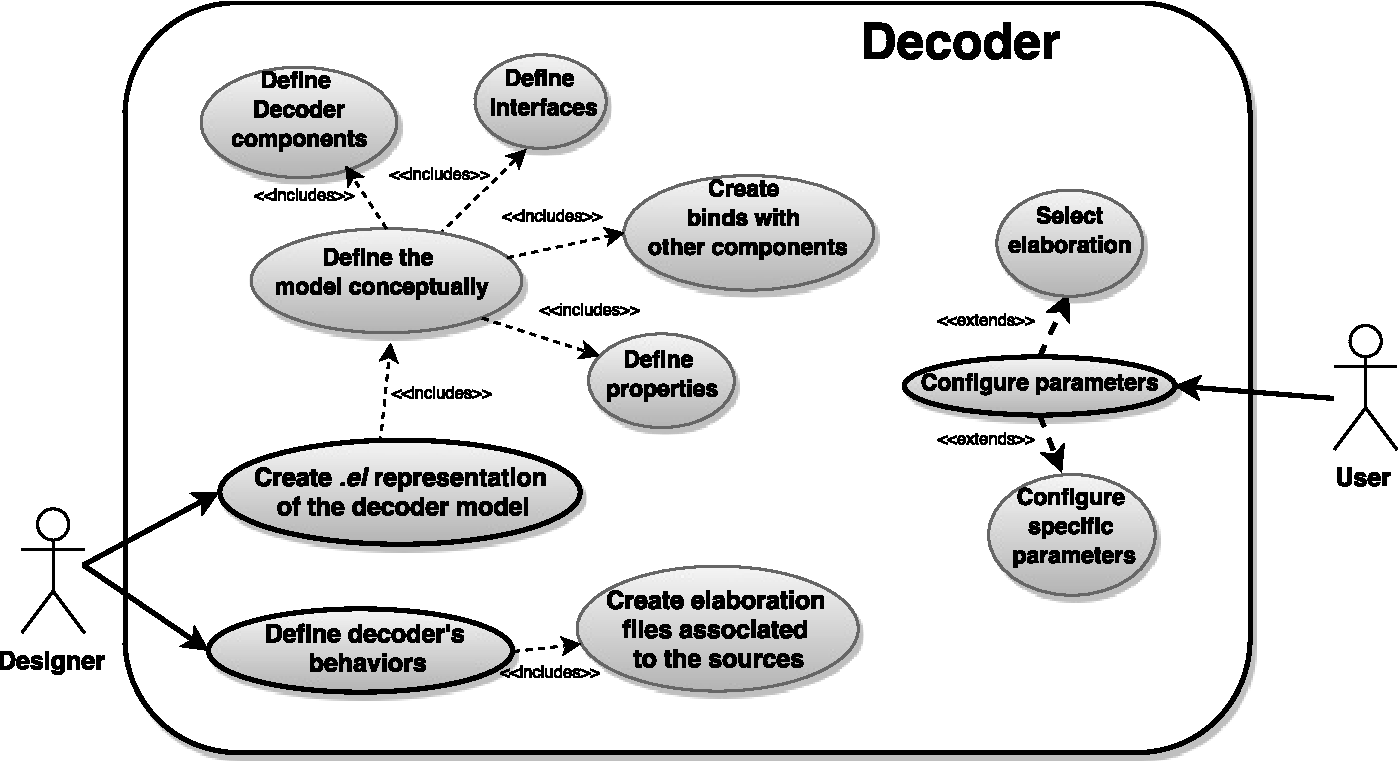
\includegraphics[scale=0.65]{images/Decoder_UseCases.pdf} }
\caption{Decoder Use Cases.}
\label{fig:DecoderUseCases} 
\end{figure}

As figure \ref{fig:DecoderUseCases} shows, the designer has similar tasks as in the DBT: define the Decoder model and create its EL representation. Although, since new implementations can be added, an elaboration file must be created for each one. The role of the user is also the same, the configuration of parameters, however, for new implementations there are some specific properties that must be chosen.
